% !TEX program = xelatex
% !BIB program = bibtex

\documentclass[screen,17pt,cn,founder,mtpro2]{elegantnote}

\usepackage{hyperref, subcaption, gbt7714}
\title{基于深度学习的行为识别数据分析 \\ ------\large{ “深度学习入门及 Python 训练” 课程报告}}
\author{龚梓阳}
\date{\zhtoday}

\begin{document}

\maketitle
\clearpage

\section{数据介绍}

\begin{figure}[hpt]
    \centering
    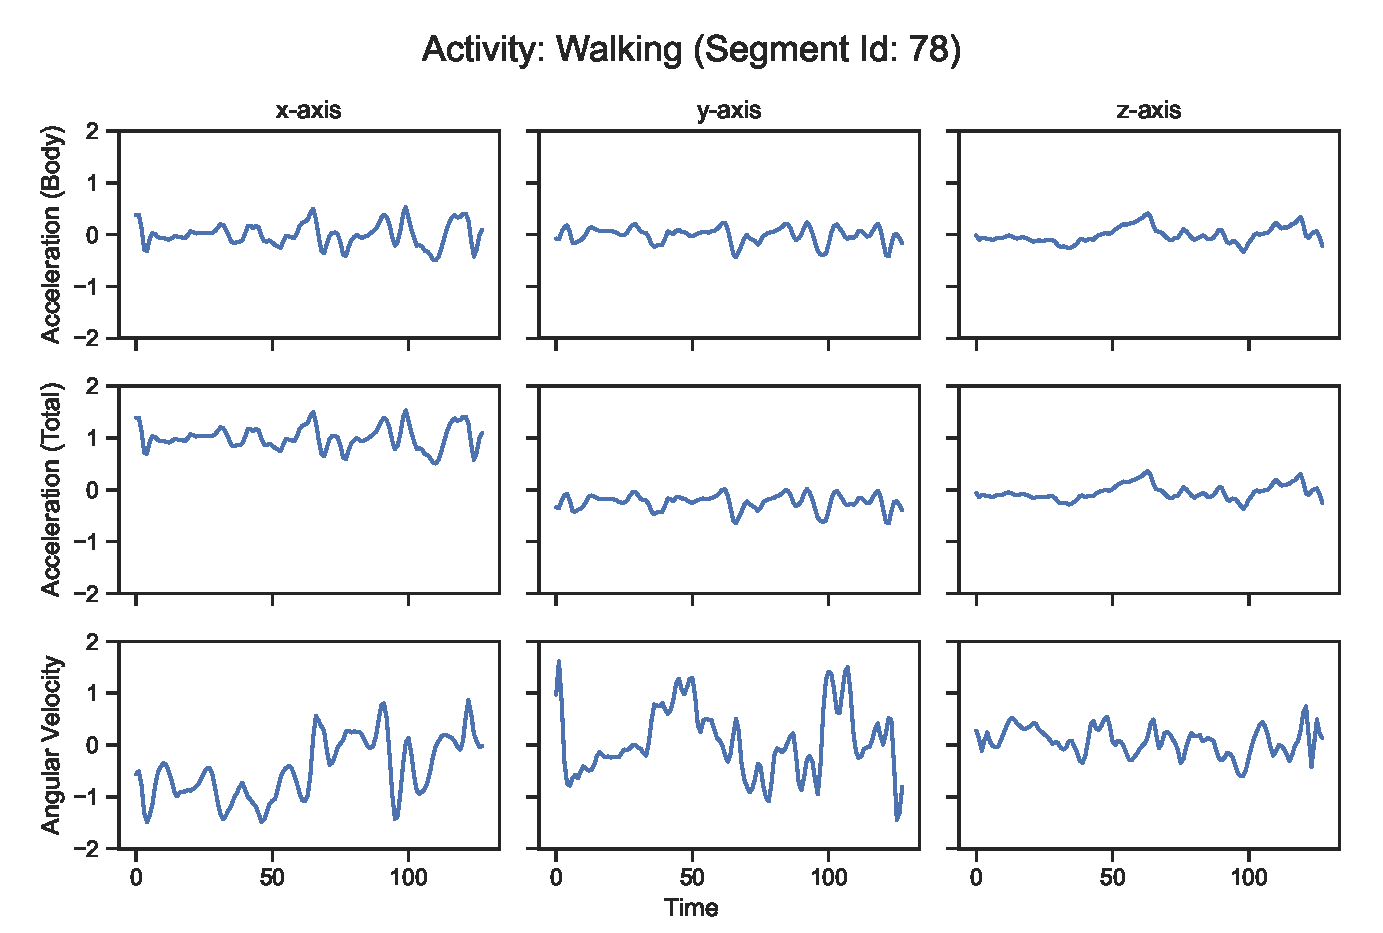
\includegraphics[width=.7\linewidth]{images/activity-walking-segment-78.eps}
    \caption{指定时间内完成指定行为(步行)的智能手机传感器数据记录\citep{anguita_public_2013}}
\end{figure}

\begin{figure}
    \begin{subfigure}{.33\textwidth}
        \centering
        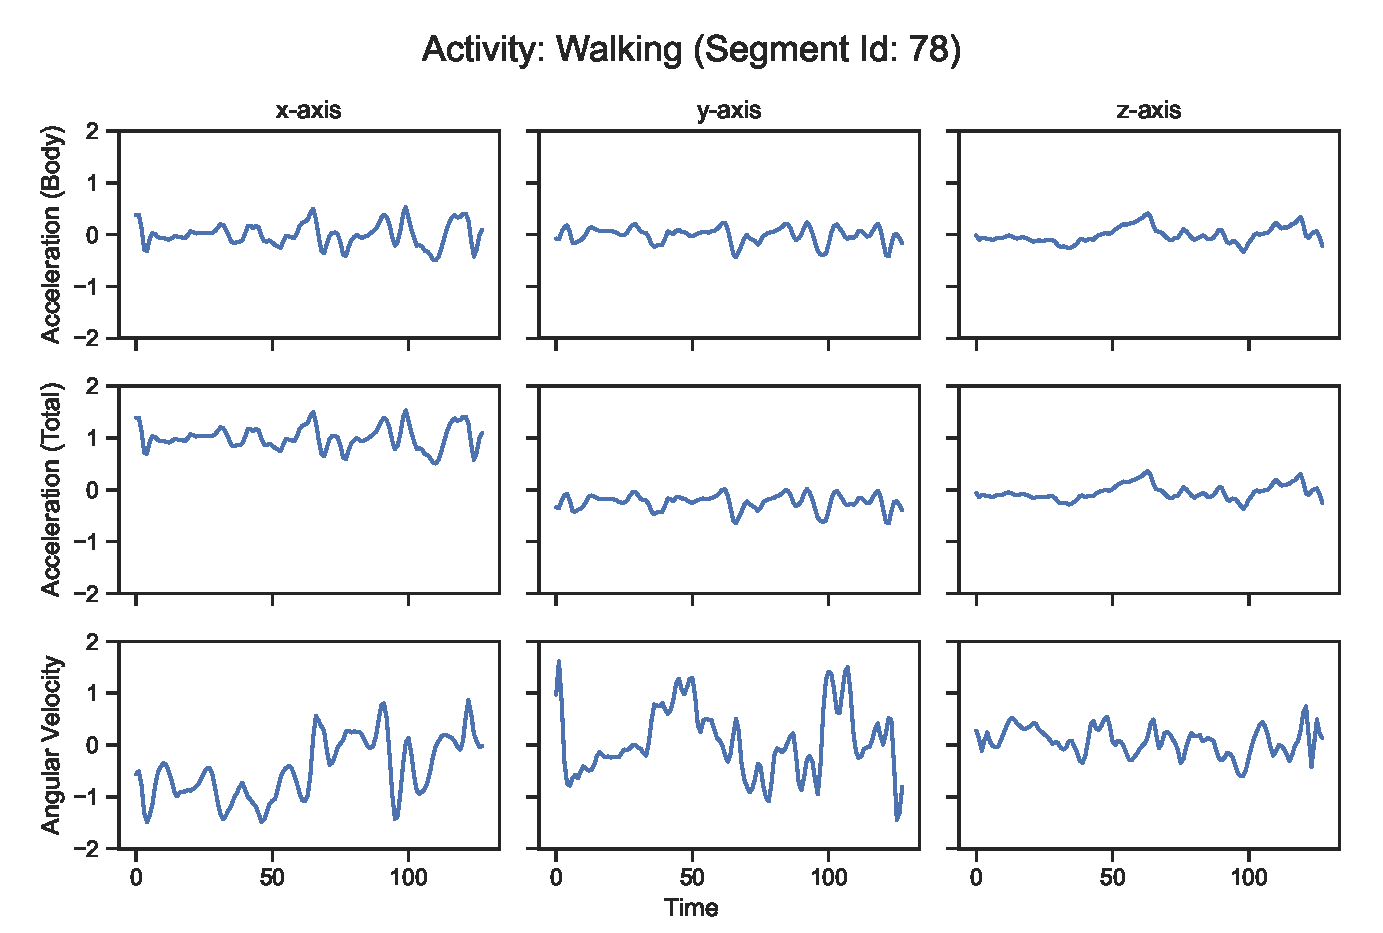
\includegraphics[width=\linewidth]{images/activity-walking-segment-78.eps}
        \caption{步行}
    \end{subfigure}
    \begin{subfigure}{.33\textwidth}
        \centering
        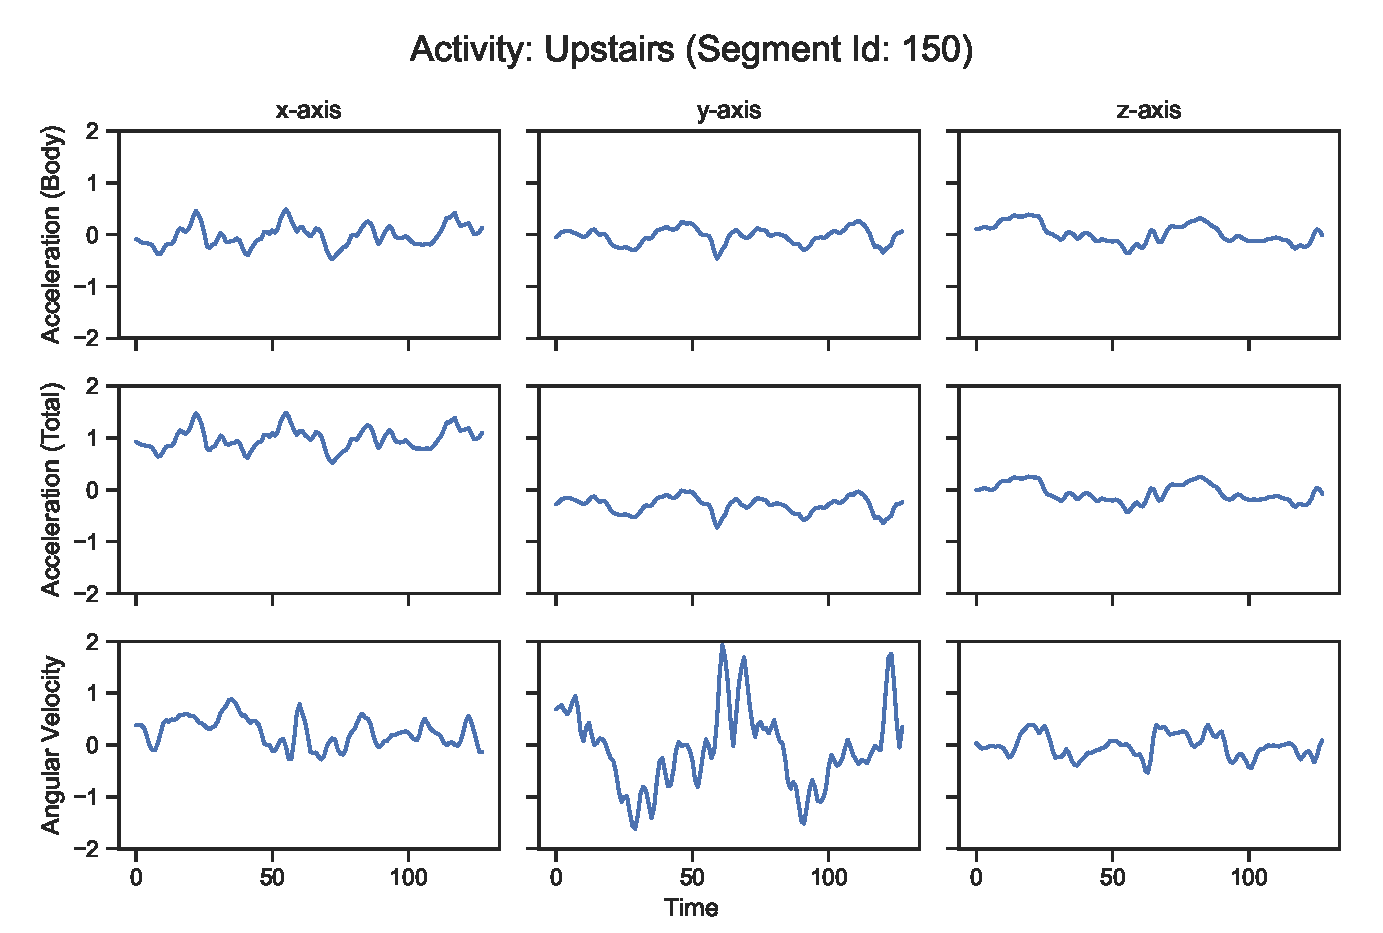
\includegraphics[width=\linewidth]{images/activity-upstairs-segment-150.eps}
        \caption{上楼}
    \end{subfigure}
    \begin{subfigure}{.33\textwidth}
        \centering
        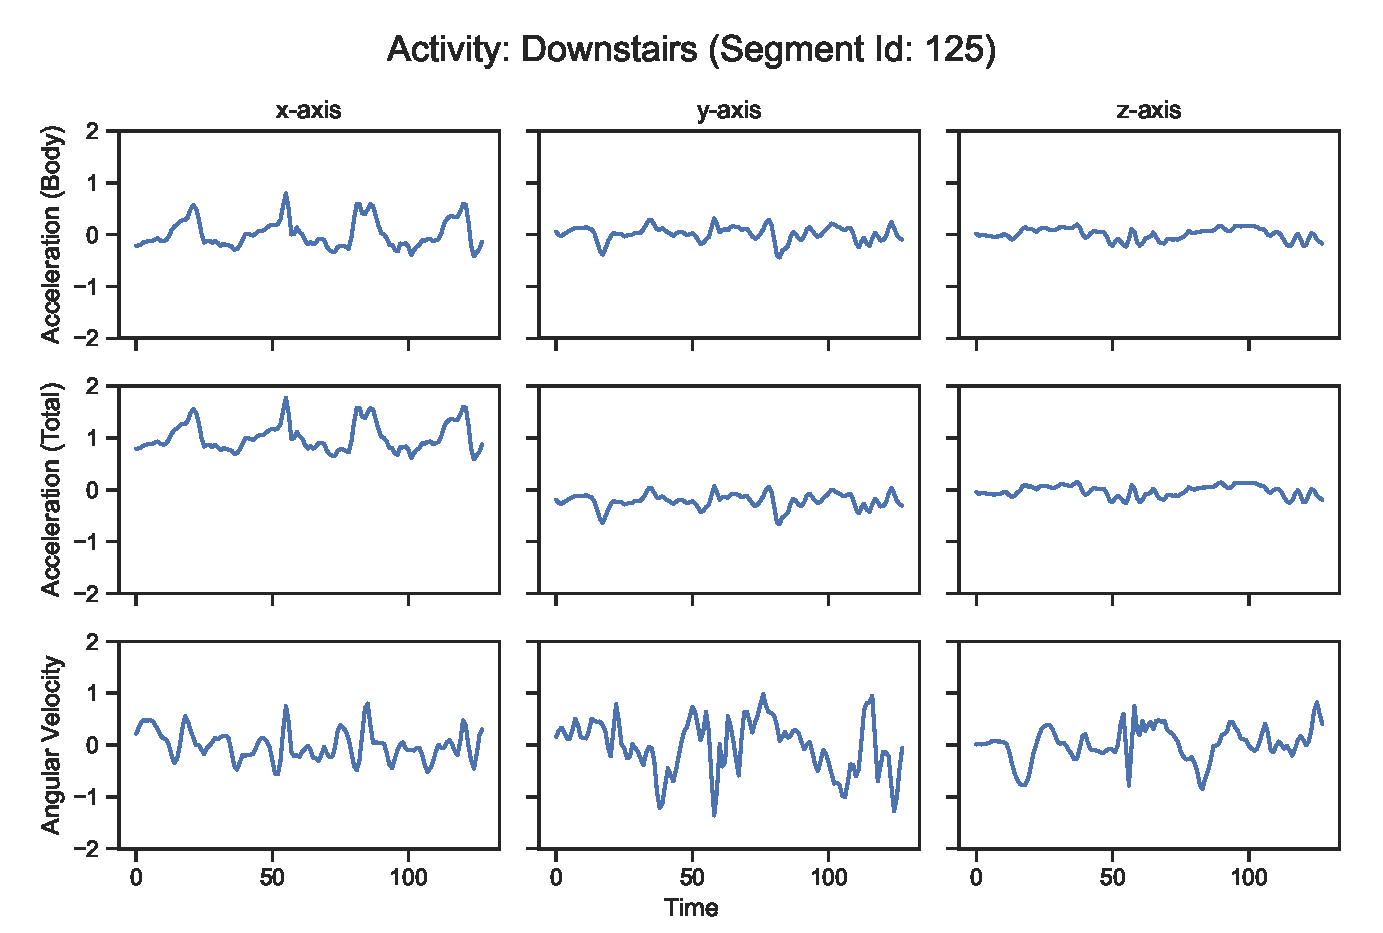
\includegraphics[width=\linewidth]{images/activity-downstairs-segment-125.eps}
        \caption{下楼}
    \end{subfigure}
    \begin{subfigure}{.33\textwidth}
        \centering
        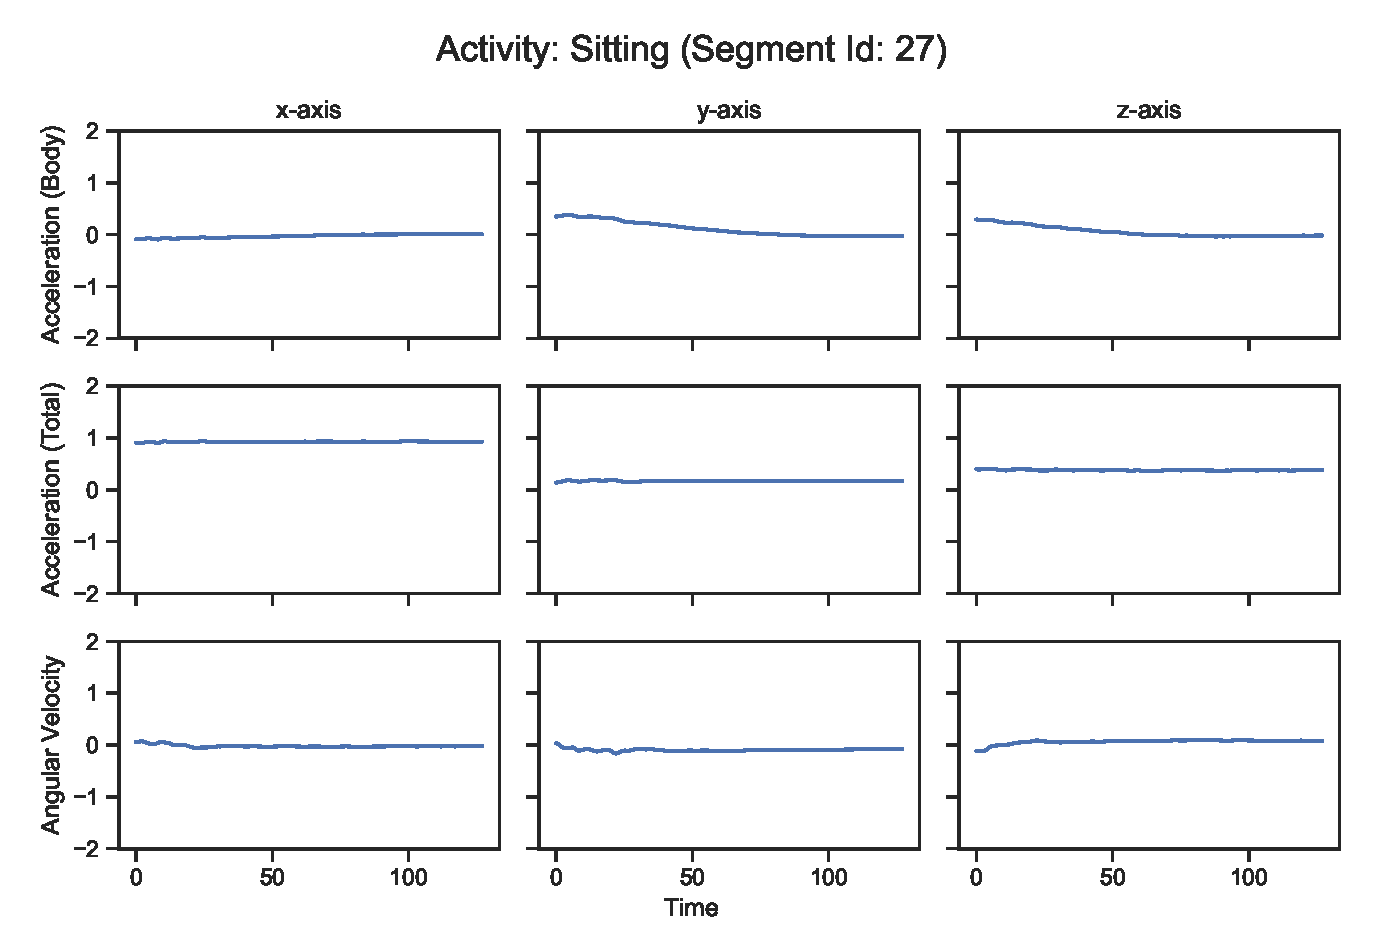
\includegraphics[width=\linewidth]{images/activity-sitting-segment-27.eps}
        \caption{静坐}
    \end{subfigure}
    \begin{subfigure}{.33\textwidth}
        \centering
        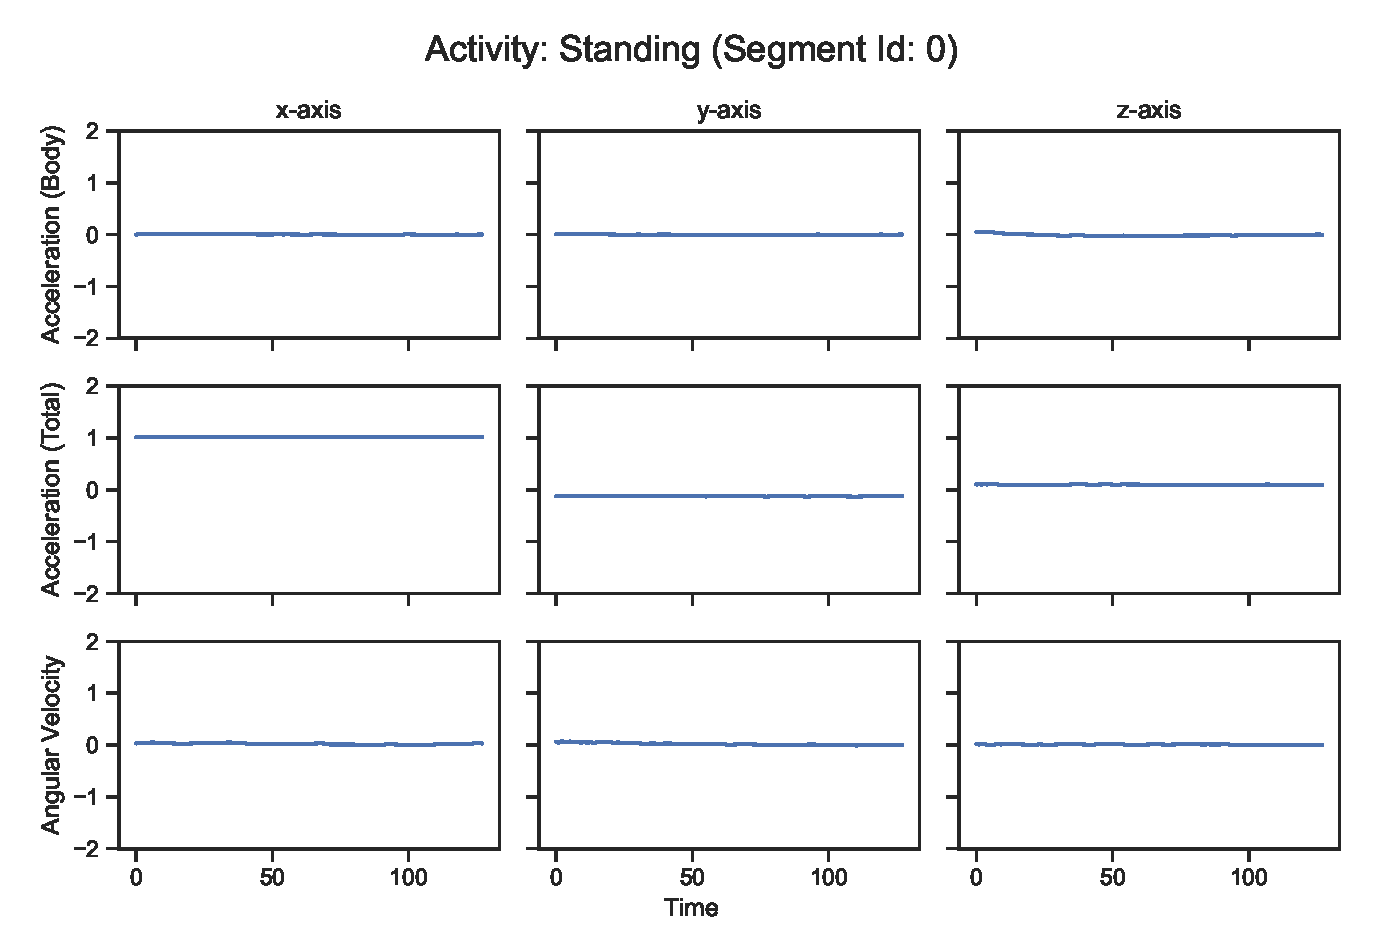
\includegraphics[width=\linewidth]{images/activity-standing-segment-0.eps}
        \caption{站立}
    \end{subfigure}
    \begin{subfigure}{.33\textwidth}
        \centering
        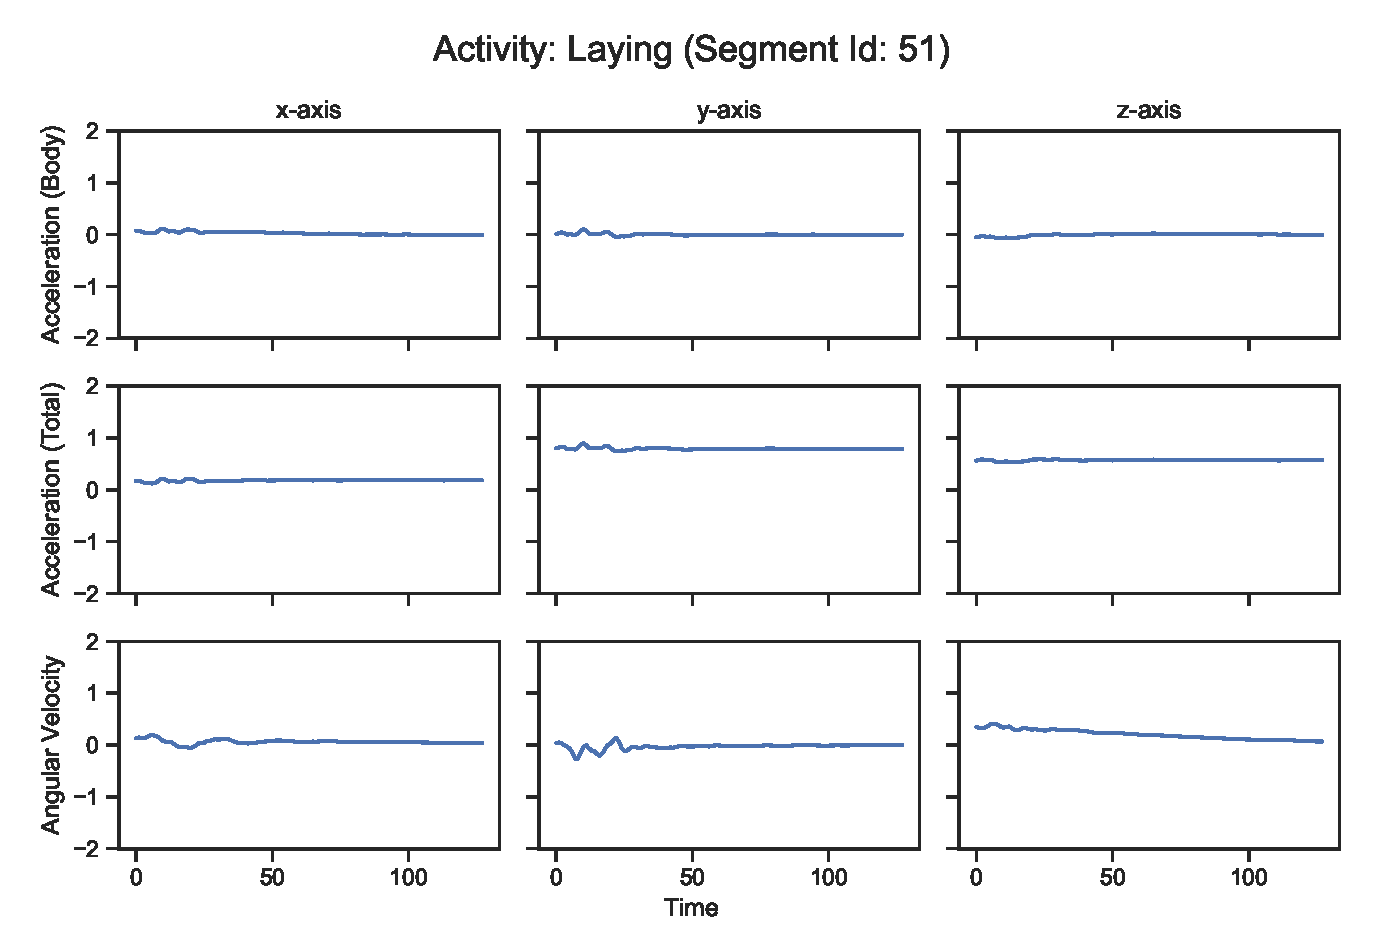
\includegraphics[width=\linewidth]{images/activity-laying-segment-51.eps}
        \caption{平躺}
    \end{subfigure}
    \caption{指定时间内完成不同指定行为(步行,上楼,下楼,静坐,站立和平躺)的智能手机传感器数据记录}
\end{figure}
\clearpage

\section{模型构建}

\begin{figure}[hpt]
    \centering
    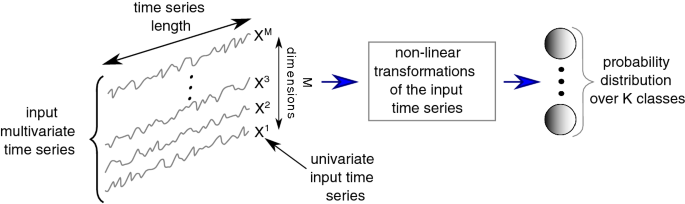
\includegraphics[width=.9\linewidth]{images/general-deep-learning-for-time-series-classification.png}
    \caption{针对时间序列数据分类的通用深度学习框架\citep{ismail_fawaz_deep_2019}}
\end{figure}

\subsection{基于统计特征的机器学习模型}

根据文献 \cite{anguita_human_2012} 中所构建的 561 个基于时域特征及频域特征的变量,包括基于多种滤波器及快速傅里叶变换所构建的统计特征。在此基础上,考虑使用 K 近邻、朴素贝叶斯、决策树、支持向量机和随机森林等潜在模型。
\clearpage

\subsection{基于 LSTM 的深度学习模型}

由于 LSTM 模型可以很好地捕捉时序数据中的信号,因此,在此处我们不做任何预处理,直接将数据放入模型之中。

\begin{figure}[hpt]
    \centering
    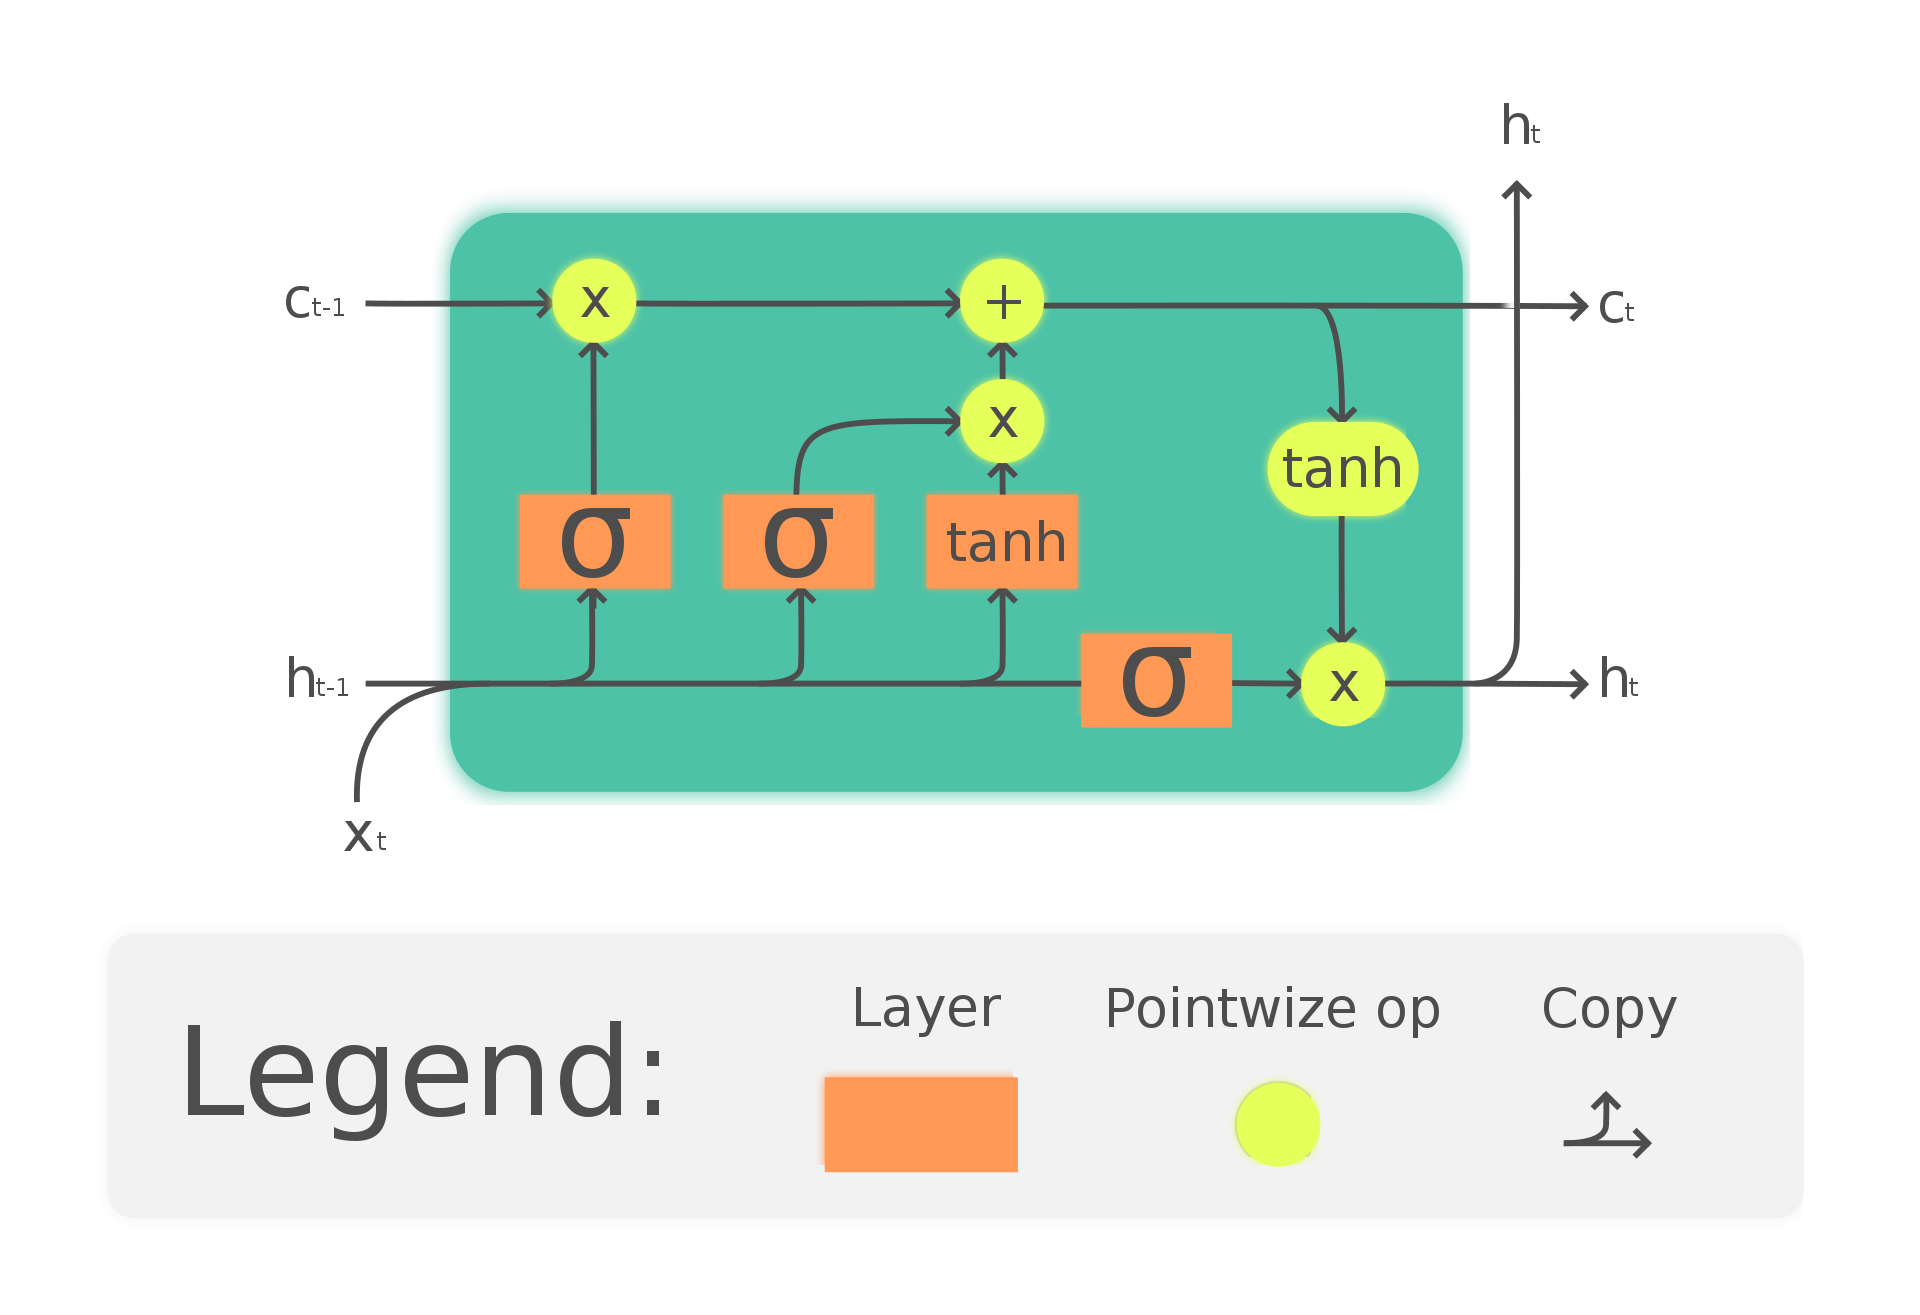
\includegraphics[width=.5\linewidth]{images/lstm-cell.png}
    \caption{LSTM (Long short-term memory) 模型}
\end{figure}

\begin{note}
    "\href{https://www.pytorchlightning.ai/}{Pytorch-Lightning}" 重构你的 PyTorch 代码,抽出复杂重复部分,让你专注于核心的构建,让你的实验更快速更便捷地开展迭代。参考示例:\href{https://github.com/SignorinoY/immortal-python}{SignorinoY/immortal-python}
\end{note}

\begin{figure}
    \centering
    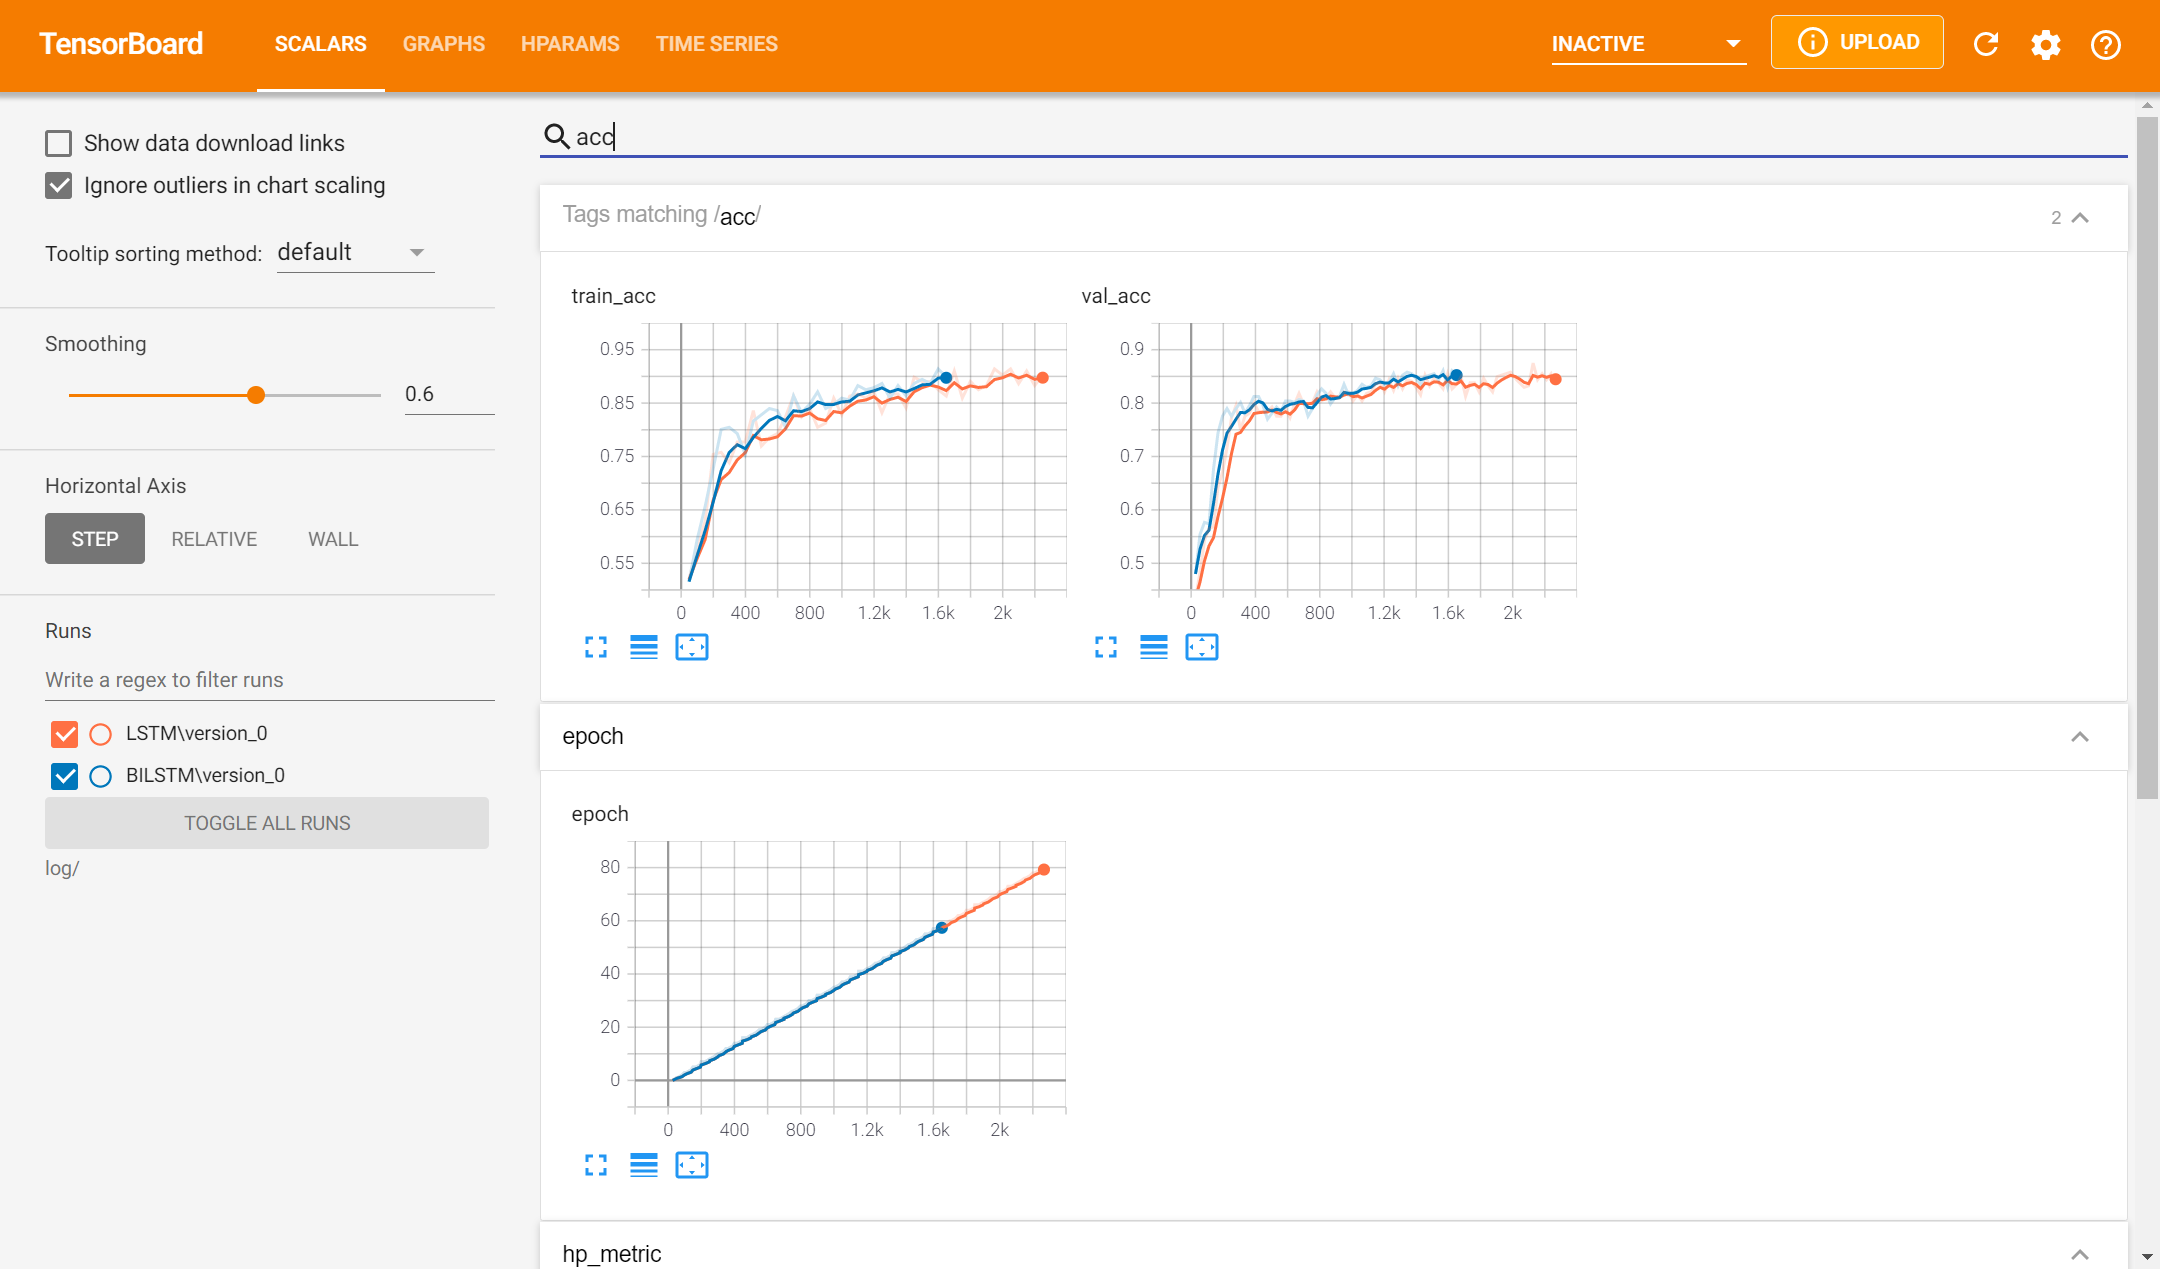
\includegraphics[width=.9\linewidth]{images/screenshots-of-tensorboard.png}
    \caption{TensorBoard 实时运行截图}
\end{figure}
\clearpage

\section{模型评价}

在均使用模型默认参数的情况下,基于同一训练集(样本量:7352)进行训练,并在同一测试集(样本量:2947)上进行预测,评价模型的预测效果。

\begin{table}[hpt]
    \centering
    \begin{tabular}{ccc|ccc}
        \toprule
        模型       & 准确率  & Macro F1 & 模型     & 准确率  & Macro F1 \\
        \midrule
        K 近邻     & 90.16\% & 0.90     & 随机森林 & 92.60\% & 0.93     \\
        朴素贝叶斯 & 77.02\% & 0.77     & LSTM     & 71.50\% & 0.71     \\
        决策树     & 85.65\% & 0.86     & BiLSTM   & 73.29\% & 0.72     \\
        支持向量机 & 95.05\% & 0.95     &                               \\
        \bottomrule
    \end{tabular}
    \caption{同一测试集下, 不同模型的预测结果}
\end{table}

此项目代码在 \href{https://github.com/SignorinoY/corruptor}{SignorinoY/corruptor} 处可见。
\clearpage

\bibliography{reference}
\end{document}